

\chapter{Introduction}

%\label{chap:GettingStarted}
\section{Overview}
The introduction of a Co-operative Society Management System marks a significant leap
in the efficient and organized management of Co-operative societies. Co-operative
societies play a vital role in various sectors, including agriculture, finance, and housing,
by fostering collaboration among members and promoting economic development.
However, managing the diverse functions and operations of these societies can be
complex and demanding. This introduction provides an overview of the purpose, features,
and benefits of such a system.

\subsection{Purpose}
The Co-operative Society Management System is meticulously crafted to cater to the distinctive needs and challenges encountered by Co-operative societies. Its core objective is to simplify and automate the administrative, financial, and member-centric processes within a Cooperative society. Through this, the system aims to elevate efficiency, transparency, and overall performance, providing a comprehensive solution tailored to the intricate requirements of Co-operative societies.

% \section{Motivation}

% \subsection{Image Processing}



\section{The History of Co-operative Societies in Bangladesh}

The concept of Co-operative societies has a deep-rooted history in Bangladesh, dating back to the pre-independence period and gaining significant momentum in the post-independence era. Here's a brief background on Co-operative societies in Bangladesh:

\subsection{Pre-independence Period}

Co-operative societies in what is now Bangladesh can trace their origins to the British colonial period. During this time, Co-operative movements began to take shape, primarily in rural areas. These early Co-operatives aimed to address the economic challenges faced by farmers and rural communities. However, the concept remained somewhat limited in scope.

\subsection{Post-independence Era}

After gaining independence from Pakistan in 1971, Bangladesh faced numerous socio-economic challenges. Co-operatives were seen as a means to empower rural communities, alleviate poverty, and promote economic development. The government of Bangladesh began to actively promote and support Co-operative initiatives as part of its socioeconomic development strategy.

Co-operative societies in Bangladesh have a diverse history and have played a significant role in addressing rural and urban development challenges. With ongoing efforts to overcome challenges and promote transparency, Co-operatives continue to be a valuable instrument for socio-economic development and poverty reduction in the country.



\section{Aims of Co-operative Societies in Bangladesh}

The aims of Co-operative societies in Bangladesh are multifaceted and are aligned with socio-economic development, poverty reduction, and the empowerment of various segments of society. Here are the primary aims of Co-operative societies in Bangladesh:

\begin{enumerate}
    \item \textbf{Poverty Alleviation}
    \item \textbf{Rural Development}
    \item \textbf{Agricultural Advancement}
    \item \textbf{Financial Inclusion}
    \item \textbf{Empowerment of Women}
    \item \textbf{Housing and Urban Development}
    \item \textbf{Entrepreneurship Development}
    \item \textbf{Social Welfare}
    \item \textbf{Community Building}
    \item \textbf{Good Governance}
\end{enumerate}

Co-operative societies in Bangladesh have a broad spectrum of aims, all of which are geared towards socio-economic development, poverty reduction, and the empowerment of individuals and communities. They play a crucial role in addressing the diverse needs of their members and contribute to the overall development of the country.


\section{Motivation}

The motivation behind developing a Co-operative Society Management System stems from the recognition of several pressing needs and challenges within Co-operative societies. Here are the primary motivations:

\begin{enumerate}
    \item \textbf{Efficiency Enhancement:} Traditional methods of managing Co-operative societies often involve manual paperwork, which can be time-consuming and error-prone. The motivation is to streamline operations and reduce administrative burdens by automating various tasks, ultimately improving efficiency.
    
    \item \textbf{Transparency and Trust:} Co-operative societies rely on the trust and cooperation of their members. By implementing a management system, societies aim to enhance transparency in financial transactions, member interactions, and decision-making processes. This increased transparency fosters trust among members and stakeholders.
    
    \item \textbf{Compliance and Reporting:} Many Co-operative societies are subject to regulatory requirements and reporting standards. A management system simplifies compliance by generating accurate financial reports and statements, making it easier to adhere to legal obligations.
    
    \item \textbf{Member Empowerment:} Co-operative societies exist for the benefit of their members. By providing an online platform for members to access their account statements, apply for loans, and engage in discussions, the system empowers members and improves their overall experience.
    
    \item \textbf{Data Security:} Data security and privacy are paramount. With the rise in cyber threats, a motivation for implementing a management system is to ensure that sensitive member and financial data is securely stored, reducing the risk of data breaches.
    
    \item \textbf{Scalability:} As Co-operative societies grow, the need for efficient management becomes more critical. The system allows for scalability, enabling societies to accommodate a larger membership base and increasing volumes of financial transactions.
    
    \item \textbf{Cost Reduction:} While there may be an initial investment in implementing the system, the long-term motivation is cost reduction. By automating tasks and reducing the need for extensive manual labor, Co-operative societies can save both time and money.
\end{enumerate}

The motivation for a Co-operative Society Management System lies in its ability to address the unique challenges faced by Co-operative societies, improve operational efficiency, enhance transparency, ensure accurate financial management, empower members, and ultimately contribute to the long-term sustainability and success of these Co-operative organizations.


% \begin{figure}
%     \centering
%     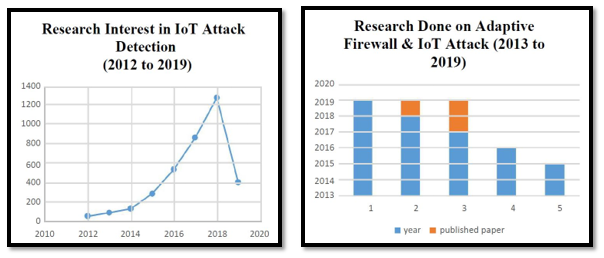
\includegraphics[scale=0.5]{Chap1/motivation.PNG}
%     \caption{Research Interest in Field of IoT}
%     \label{fig:motivation}
% \end{figure}

%  In figure \ref{fig:motivation} shows the existing research interest in IoT Attack Detection which is increasing day by day for last few years whereas for detecting attack concept of Adaptive Firewall is not so common and used term in this field. This drives us motivated to design adaptive firewall for attack detection and to block illegitimate traffic on IoT Network Model.

\section{Findings of Our Study}

Cooperative society is an association where the members voluntarily cooperate for mutual social, cultural, and economic benefit. The study reveals the following scenarios regarding how the cooperative societies in Dhaka are operating, how the members are cooperating for their mutual benefit, and how they are contributing to the socio-economic benefit of Bangladesh:

\begin{figure}[h]
    \centering
    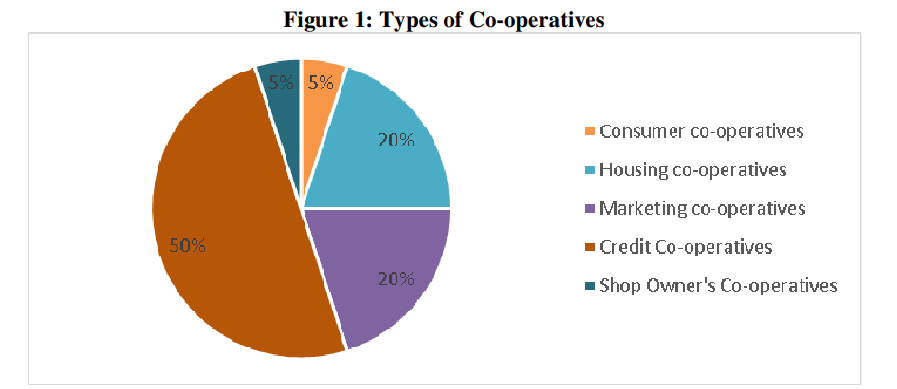
\includegraphics[width=0.6\textwidth]{Chap1/figure1.PNG}
    % \caption{Caption for your image.}
    \label{fig:example}
  \end{figure}

  Inference: The figure 1 shows that out of 20 Cooperatives, 5 percent Cooperatives are Consumer Cooperatives, 
  20 percent are Housing Cooperatives, 20 percent are Marketing Cooperatives, 50 percent are Credit 
  Cooperatives and 5 percent are Shop Owner’s Cooperatives in Dhaka. 
  
  \begin{figure}[h]
    \centering
    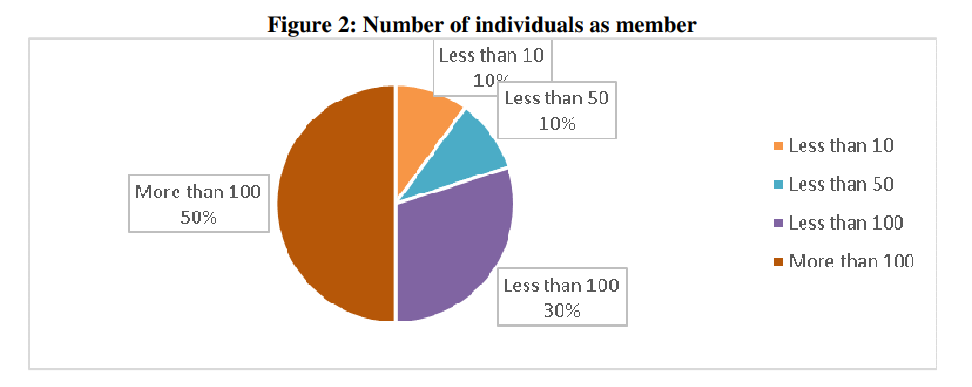
\includegraphics[width=0.6\textwidth]{Chap1/figure2.PNG}
    % \caption{Caption for your image.}
    \label{fig:example}
  \end{figure}

  Inference: The figure 2 shows that out of 20 cooperatives , 10 percent cooperatives have members of less than 
10, 10 percent cooperatives have members of less than 50, 30 percent cooperatives have members of less than 
100, 50 percent cooperatives have members of more than 100. 

\begin{figure}[h]
    \centering
    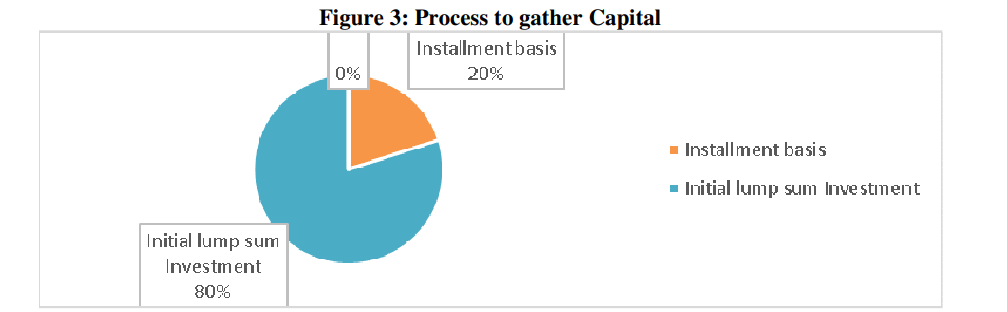
\includegraphics[width=0.6\textwidth]{Chap1/figure3.PNG}
    % \caption{Caption for your image.}
    \label{fig:example}
  \end{figure}

  Inference: The figure 3 shows that out of 20 cooperatives, 20 percent cooperatives collect their capital as 
installment basis (most of the cases monthly installment) and 80 percent cooperatives collect their capital at the 
time of launching the cooperatives as initial lump sum investment. 

\begin{figure}[h]
    \centering
    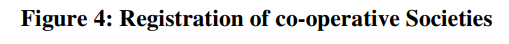
\includegraphics[width=0.6\textwidth]{Chap1/figure4.1.PNG}
    % \caption{Registration of co-operative Societies}
    \label{fig:example}
    \centering
    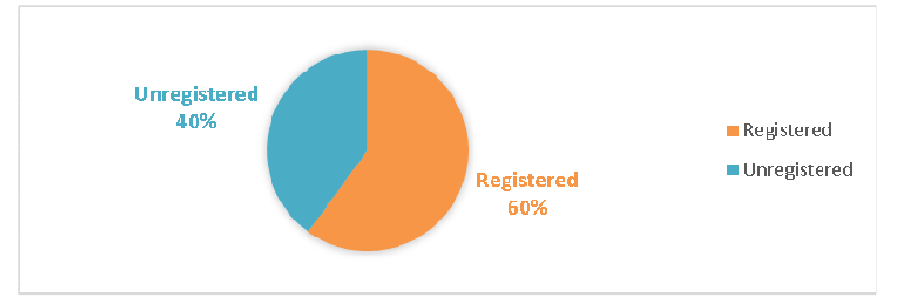
\includegraphics[width=0.6\textwidth]{Chap1/figure4.PNG}
    % \caption{Registration of co-operative Societies}
    \label{fig:example}
  \end{figure}

  Inference: The figure 4 shows that out of 20 cooperatives, 40 percent cooperatives are operating their
organization without taking registration from the concerned authority because the registration process is not easy 
due to bureaucratic problem and 60 percent co-operatives are operating by taking the registration.

\begin{figure}[h]
    \centering
    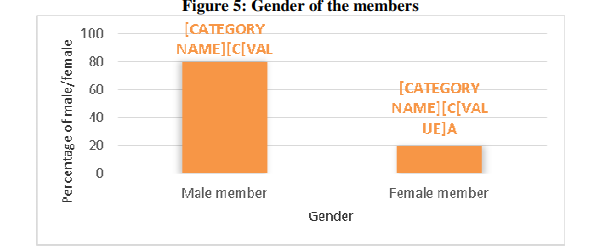
\includegraphics[width=0.6\textwidth]{Chap1/figure5.PNG}
    % \caption{Caption for your image.}
    \label{fig:example}
  \end{figure}

  Inference: The figure 5 shows that among the members in the cooperatives only 20\% members are female and 80\% members are male. So it is clear that the female participation is lower than the male participation in the cooperatives.

  \begin{figure}[h]
    \centering
    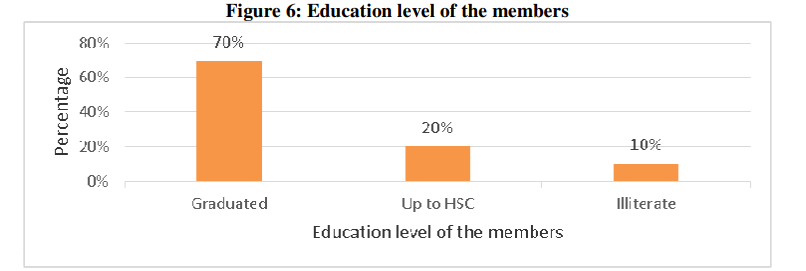
\includegraphics[width=0.6\textwidth]{Chap1/figure6.PNG}
    % \caption{Caption for your image.}
    \label{fig:example}
  \end{figure}

  Inference: The figure 6 shows that among the members in the cooperatives, 70\% are graduates, 20\% have passed up to HSC, and 10\% are illiterate.
  
  \begin{figure}[h]
    \centering
    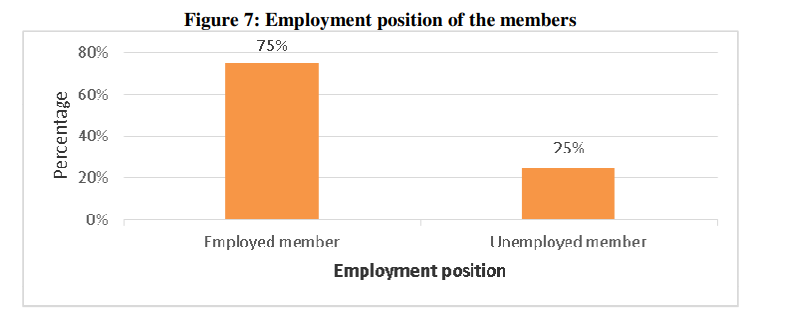
\includegraphics[width=0.6\textwidth]{Chap1/figure7.PNG}
    % \caption{Caption for your image.}
    \label{fig:example}
  \end{figure}

  Inference: The figure 7 shows that among the members in the co-operatives 75\%members are employed, 25\% members are unemployed. 

  \begin{figure}[h]
    \centering
    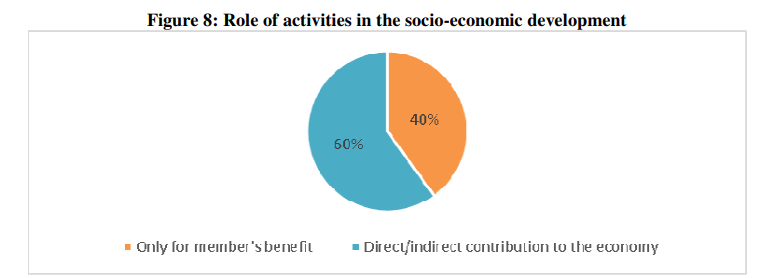
\includegraphics[width=0.6\textwidth]{Chap1/figure8.PNG}
    % \caption{Caption for your image.}
    \label{fig:example}
  \end{figure}

  Inference: The figure 8 illustrates that among the 20 cooperatives surveyed:

  \begin{itemize}
      \item 40\% of the cooperatives believe that their activities primarily benefit their members. Additionally, they express the belief that these activities may indirectly contribute to the development of the country.
      
      \item On the other hand, 60\% of the cooperatives believe that their activities directly contribute to the economic development of Bangladesh. This belief is attributed to their active participation in business-related activities.
  \end{itemize}
  

  \section{Problems of Cooperatives in Bangladesh}

The study reveals several challenges faced by cooperatives in Bangladesh:

\begin{enumerate}
    \item \textbf{Registration Challenges:}
        \begin{itemize}
            \item Many cooperatives without registration face difficulties in understanding the registration process.
            \item Bureaucratic obstacles hinder the registration process with the concerned authority.
        \end{itemize}
    
    \item \textbf{Gender Disparity:}
        \begin{itemize}
            \item Female participation in cooperatives is notably lower than male participation, impacting the true and effective realization of socio-economic benefits.
        \end{itemize}
    
    \item \textbf{Internal Conflicts:}
        \begin{itemize}
            \item Internal conflicts among cooperative members hinder progress.
            \item Predominance of vested interests within cooperatives contributes to internal conflicts.
        \end{itemize}
    
    \item \textbf{Lack of Professional Management:}
        \begin{itemize}
            \item Cooperatives suffer from a lack of professional management.
            \item Members often lack knowledge on successfully operating a cooperative.
        \end{itemize}
    
    \item \textbf{Political Interference:}
        \begin{itemize}
            \item Political interference poses a significant threat to the progress of cooperatives.
        \end{itemize}
    
    \item \textbf{Financial Constraints:}
        \begin{itemize}
            \item Limited capital supplied by members creates financial problems.
            \item Financial constraints hinder cooperatives from taking advantage of new opportunities.
        \end{itemize}
    
    \item \textbf{Lack of Motivation and Guidance:}
        \begin{itemize}
            \item Higher-level stakeholders lack motivation to highlight cooperative opportunities.
            \item Insufficient guidance is provided to obtain relative assistance from concerned authorities.
        \end{itemize}
\end{enumerate}


